
\chapter{\IfLanguageName{dutch}{Proof of Concept}{Proof of Concept}}%

\label{ch:proof-of-concept}

\section{Opbouw scenario's}

Om de \textit{Swift OpenAPI Generator} grondig te testen, concentreren we ons op een specifiek onderwerp: een boekenverlanglijst. Dit overkoepelende idee is onderverdeeld in kleinere scenario’s om het beter te kunnen uitwerken en de mogelijkheden van de \textit{Swift OpenAPI Generator} te gaan testen. 

\begin{itemize}
  \item	Scenario 1: gedeelde lijst van boeken met databaseconnectie
  \item	Scenario 2: back-end logica toevoegen voor \textit{logging}, \textit{metrics} en validatie. 
  \item Scenario 3: toevoegen van authentificatie
  \item Scenario 4: \textit{client} van de server aanmaken
  \item Scenario 5: aanpasbaarheid van back-end nadat dat er een \textit{client} is toegevoegd
\end{itemize}

\section{Scenario 1: Gedeelde lijst van boeken met databaseconnectie}
Gebruikers hebben toegang tot een gedeelde lijst van boeken, waar ze informatie over elk boek kunnen bekijken en boeken kunnen gaan toevoegen en aanpassen. Deze lijst is toegankelijk voor alle gebruikers en maakt verbinding met een databank om de boeken op te slaan en op te halen. 

\subsection{Technische doelstellingen}
De technische doelstellingen omvatten verschillende belangrijke aspecten. Allereerst moet er een OpenAPI-document gecreërd worden dat alle vereiste requestmethoden omvat, zoals POST, CREATE, UPDATE, GET en GET / ID.  Dit document bevat een gedetailleerde opsomming van hoe verzoeken geformuleerd en verwerkt moeten worden. Het is opgesteld volgens de OpenAPI-specificaties. Daarnaast is het essentieel om een stabiele en efficiënte databaseverbinding tot stand te brengen, zodat we de nodige boekgegevens kunnen opslaan en ophalen. 

Eenmaal verbonden met de databank, moet de \textit{handler} uitgewerkt worden. Deze \textit{handler} is verantwoordelijk voor het verwerken van alle inkomende verzoeken. Hierbij wordt de nodige logica toegevoegd om aan elk type verzoek correct te kunnen voldoen. Dit omvat het verwerken van verzoeken voor het toevoegen, bijwerken en opvragen van boekgegevens, evenals het ophalen van specifieke boeken op basis van hun unieke ID.


\subsubsection{Aanmaken van OpenAPI document}

Een correcte syntax is essentieel bij het opstellen van een OpenAPI-document, aangezien zelfs een kleine fout de interpretatie van de generator kan beïnvloeden. Om dergelijke fouten te voorkomen, is de OpenAPI-document gemaakt in VScode met behulp van de extensie 'vscode-openapi-viewer'. 

In een OpenAPI-document begint men met het specificeren van de versie, gevolgd door eventuele aanvullende informatie in de 'info'-sectie. Vervolgens worden de servers gedefinieerd om aan te geven op welke URL de API zal draaien.  
\begin{lstlisting}[caption=openapi.yml file]
    openapi: 3.1.0
    info:
    title: Books API
    version: 1.0.0
    servers:
    - url: 'http://localhost:8080/api'
\end{lstlisting}

Pas daarna worden de paden en endpoints van de API gespecificeerd. In een OpenAPI-document worden endpoints gedefinieerd als de verschillende paden (paths) waarop de API kan worden aangesproken. Elk pad vertegenwoordigt een bepaalde resource of functionaliteit en kan verschillende HTTP-methoden ondersteunen, zoals GET, POST, PUT, DELETE, enz. Hieronder vind je een opsomming van de verschillende request met meer uitleg per request.

\begin{itemize}
    \item	GET /Books haalt een lijst van alle boeken op. De respons is een json-array van boek objecten
\begin{lstlisting}[caption=openapi.yml file]
paths:
  /books:
    get:
      operationId: getAllBooks
      summary: Get all books
      description: Returns a list of all books
       responses:
         '200':
           description: A list of books
           content:
             application/json:
               schema:
                 type: array
                 items:
                   $ref: '#/components/schemas/Book'
     \end{lstlisting}
    \item POST /Books maakt een nieuw boek aan. Het request moet een json-object bevatten met de informatie van het nieuwe boek, de respons geeft het aangemaakte boek terug
\begin{lstlisting}[caption=openapi.yml file]
    post:
      operationId: createBook
      summary: Create a new book
      description: Creates a new book
      requestBody:
        content:
          application/json:
            schema:
              $ref: '#/components/schemas/Book'
      responses:
        '201':
          description: The created book
          content:
            application/json:
              schema:
                $ref: '#/components/schemas/Book'
        
    \end{lstlisting}
    \item GET /books/{id} haalt de gegevens terug van één specifiek boek door het Id, een path parameter, te gebruiken. 
    \begin{lstlisting}[caption=openapi.yml file]
  /books/{id}:
    get:
      operationId: getById
      summary: Get a book by ID
      description: Returns a book with the specified ID
      parameters:
        - name: id
          in: path
          description: The ID of the book
          required: true
          schema:
            type: string
    responses:
      '200':
        description: A book
        content:
          application/json:
            schema:
              $ref: '#/components/schemas/Book'
      '404':
        description: Book not found
        
    \end{lstlisting}
    \item PUT /books/{id} werkt de informatie bij van een specifiek boek door het id te gebruiken in het pad. Het request moet een JSON-object hebben met de bijgewerkte informatie, de respons is het bijgewerkte boek. 
  

\begin{lstlisting}[caption=openapi.yml file]
    put:
      operationId: updateBook
      summary: Update a book by ID
      description: Updates a book with the specified ID
      parameters:
        - name: id
          in: path
          description: The ID of the book
          required: true
          schema:
            type: string
      requestBody:
        content:
          application/json:
            schema:
              $ref: '#/components/schemas/Book'
      responses:
        '200':
          description: The updated book
          content:
            application/json:
              schema:
                $ref: '#/components/schemas/Book'
\end{lstlisting}

\end{itemize}
Helemaal onderaan, na de specificatie van de paden en \textit{endpoints}, volgt de sectie voor het definiëren van de \textit{components}. Deze \textit{components} zijn herbruikbare elementen binnen het OpenAPI-document. Dit kunnen schema's voor gegevensstructuren, parameters, en antwoorden op verzoeken zijn. Door componenten te gebruiken, kunnen we duplicatie verminderen en consistentie waarborgen in het hele document.

\begin{lstlisting}[caption=openapi.yaml file]
components:
  schemas:
    Book:
      type: object
      properties:
        id:
          type: string
          description: The ID of the book
        title:
          type: string
          description: The title of the book
        author:
          type: string
          description: The author of the book
required:
  - id
  - title
  - author
\end{lstlisting}




\subsubsection{Verbinding met databank}

Bij de eerste poging om verbinding te maken met de databank, werd er het voorbeeld gebruikt dat beschikbaar was op de Git-repository van de \textit{Swift OpenAPI Generator}. Maar al snel werd duidelijk dat dit voorbeeld veel te \textit{low-level} was. Het maakt de code complex en ingewikkeld, waardoor het lastig was om een efficiënte databank verbinding tot stand te brengen die kon herbruikt worden.  
Er werd over-gegaan naar meer vertrouwde methoden. Er werd geprobeerd om de connectie op te zetten zoals gebruikelijk is bij het ontwikkelen van back-endsystemen.  \\ 

Zo is de databank toegevoegd aan de \textit{main server} van de applicatie. Zodat deze onmiddellijk wordt opgezet als de applicatie runt. Om de databank operationeel te maken en de benodigde tabellen toe te voegen, is er gebruik gemaakt van \textit{migrations}. Door \textit{migrations} te gebruiken, kunnen er gemakkelijk wijzigingen in de databasestructuur doorgevoerd worden en deze synchroniseren met de applicatiecode. Dit garandeert een consistente en betrouwbare databaseconfiguratie.
\begin{lstlisting}[caption=Migration file]
   import Fluent
   struct CreateBooks: AsyncMigration {
       func prepare(on database: FluentKit.Database) async throws {
           return try await database.schema("books")
           .id()
           .field("title", .string, .required)
           .field("author", .string)
           .create()
       }
       
       func revert(on database: FluentKit.Database) async throws {
           try await database.schema("books").delete()
       }
   } 
\end{lstlisting}

Daarnaast zijn er  models gemaakt voor de gegevens die in de databank worden opgeslagen. Dit werd zo gedaan omdat de standaard datatypen van een OpenAPI-document niet rechtstreeks aan de databank kon worden toegevoegd. Dit betekent dat wanneer er een verzoek wordt gedaan aan de applicatie, de gegevens die worden ontvangen eerst moeten worden aangepast naar het juiste gegevenstype.

\begin{lstlisting}[caption=Model file]
final class Book: Model, Content {
    static let schema = "books"
    @ID(key: .id)
    var id: UUID?
    @Field(key: "title")
    var title : String
    @Field(key: "author")
    var author : String
    
    init() { }
    
    init(id: UUID? = nil, title: String, author: String) {
        self.id = id
        self.title = title
        self.author = author
    }
}
\end{lstlisting}

In traditionele back-end systemen is het mogelijk om de databank op te halen aan de hand van het \textit{Request} dat je ontvangt, maar tegen initiële verwachtingen in werkte dit niet met de \textit{Swift OpenAPI Generator}. Dit komt doordat de \textit{Swift OpenAPI Generator} zelf een APIProtocol heeft, wat een extra laag van complexiteit toevoegt. Concreet betekent dit dat de gebruikelijke methoden om de databank op te halen niet functioneerden zoals anders. Om dit op te lossen, wordt simpelweg de databank door gegeven van de server aan de \textit{handler}. Dit was een effectieve oplossing die ervoor zorgde dat de databank toegankelijk was zonder te interfereren met de werking van de \textit{Swift OpenAPI Generator}.

\begin{lstlisting}[caption=booksServiceServer file]
@main struct booksServiceServer {
    static func main() async throws {
        
        let app = Vapor.Application()
        app.databases.use(DatabaseConfigurationFactory.postgres(configuration: .init(
        hostname: Environment.get("DATABASE_HOST") ?? "localhost",
        port: Environment.get("DATABASE_PORT").flatMap(Int.init(_:)) ?? SQLPostgresConfiguration.ianaPortNumber,
        username: Environment.get("DATABASE_USERNAME") ?? "vapor_username",
        password: Environment.get("DATABASE_PASSWORD") ?? "vapor_password",
        database: Environment.get("DATABASE_NAME") ?? "vapor_database",
        tls: .prefer(try .init(configuration: .clientDefault)))
        ), as: .psql)
        
        app.migrations.add(CreateBooks())
        try app.autoMigrate().wait()
        
        let transport = VaporTransport(routesBuilder: app)
        let handler = Handler(app: app)
        try handler.registerHandlers(on: transport, serverURL: URL(string: "/api")!)
        try await app.execute()
    }

\end{lstlisting}

\subsubsection{Toevoegen van de \textit{handler}}
Nadat de verbinding met de databank tot stand is gebracht, is het noodzakelijk om de verzoeken vanuit het OpenAPI-document nog te verwerken. Deze verwerking wordt doorgaans uitgevoerd in de \textit{handler} van de applicatie. De \textit{handler} fungeert als een tussenliggende laag tussen de ontvangen verzoeken en de daadwerkelijke verwerking ervan.
Binnen de \textit{handler} worden de ontvangen verzoeken geanalyseerd, gevalideerd en doorgegeven aan de databank. Dit omvat vaak het interpreteren van de gegevens in het verzoek, het oproepen van de bijbehorende methoden of services om de gevraagde acties uit te voeren en het afhandelen van eventuele fouten of uitzonderingen die zich tijdens dit proces kunnen voordoen. Het ontwikkelen van een efficiënte \textit{handler} is van groot belang want zonder deze \textit{handler} zal de back-end niet kunnen functioneren.  \\

De functie \textit{getAllBooks} heeft een input parameter van het type ‘\textbf{Operations.getAll-Books.Input}’. Deze parameter is een \textit{struct} die gedefinieerd is door de \textit{Swift OpenAPI Generator} en bevat informatie over de invoer van de functie. In dit geval wordt de input parameter niet gebruikt, maar moet wel worden gedefinieerd om te voldoen aan de OpenAPI-specificaties. Deze functie is in het algemeen een eenvoudige functie die alle boeken van uit een databank ophaalt en retourneert als een array van \textbf{Components.Schemas.Book} objecten. 
\begin{lstlisting}[caption=handler file - getAllBooks]
func getAllBooks(_ input: Operations.getAllBooks.Input) async throws -> Operations.getAllBooks.Output {
     let books = try await Book.query(on: app.db).all()
     var booksArray: Array<Components.Schemas.Book> = []
     books.forEach { book in
          booksArray.append(Components.Schemas.Book(id: "\(String(describing: book.id))", title: book.title, author: book.author))
     }
     return .ok(.init(body: .json(booksArray)))
}
        

\end{lstlisting}
De volgende functie \textit{getById} heeft een parameter van het type ‘\textbf{Operations.getById.\\Input}’. Deze parameter is in deze functie van belang om het juiste boek op te halen. De regel let id = UUID(uuidString: input.path.id) haalt het id van het boek op uit de invoerparameter. ‘path’ bevat informatie over de padparameters die in een API-aanroep kan aanwezig zijn. In dit geval bevat deze één eigenschap ‘id’ van het type string. Vervolgens wordt het gevraagde boek opgehaald uit de databank aan de hand van het \textit{‘Book’}- model. Als laatste moet het boek omgezet worden naar het type \textbf{‘Components.Schemas.Book’}.

\begin{lstlisting}[caption=handler file - getById]
func getById(_ input: Operations.getById.Input) async throws -> Operations.getById.Output {
    let id = UUID(uuidString: input.path.id)
    guard let book = try await Book.find(id, on: app.db) else {
        throw Abort(.notFound)
    }
        
    return .ok(.init(body: .json(Components.Schemas.Book(id: "\(String(describing: book.id))", title: book.title, author: book.author))))
}
\end{lstlisting}

De functie \textit{createBook} maakt een nieuw boek aan, aan de hand van de input. De functie accepteert één parameter input van het type \textbf{Operations.updateBook\\.Input}, die het te wijzigen boek bevat. Deze parameter wordt gedecodeerd met een switch-statement op body, waarbij ervan wordt uitgegaan dat de body in JSON-indeling is opgegeven. Als de input een JSON-object is, zullen de gegevens worden omgezet naar een \textit{Book} element om het te kunnen toevoegen in de databank.  Vervolgens moet het \textit{book} uit de database weer worden omgezet naar een het type \textbf{‘Components.Schemas.Book’}. 

\begin{lstlisting}[caption=handler file - createBook]
func createBook(_ input: Operations.createBook.Input) async throws -> Operations.createBook.Output {
   guard case .json(let bookInput) = input.body else {
        fatalError()
    }
        
    let id = UUID(uuidString: bookInput.id)
    var book = Book(id: id, title: bookInput.title, author: bookInput.author)
    try await book.save(on: app.db)
    let bookapi: Components.Schemas.Book
    switch input.body {
        case .json(let json): bookapi = json
        case .none:
        bookapi = .init(id: "", title: "", author: "")
        break
    }
    return .created(.init(body: .json(bookapi)))
}
\end{lstlisting}
De functie \textit{updateBook} accepteert één parameter input die het te wijzigen boek bevat. Deze parameter wordt gedecodeerd met een switch-statement op \textit{body}. \textit{‘Body’} zou een JSON-object moeten bevatten van het type \textbf{‘Components.Schema.Book’}. Vervolgens wordt het id van het \textit{book} opgehaald en gebruikt om het boek te vinden in de databank.  Als het boek wel bestaat, worden de eigenschappen \textit{title} en \textit{author} bijgewerkt met de waarden uit de invoer. Vervolgens wordt het bijgewerkte boek opgeslagen in de databank met de methode \textit{update(on:)}. Ten slotte wordt het bijgewerkte boek geretourneerd als antwoord op de aanvraag, ingepakt in een JSON-object.



\begin{lstlisting}[caption=handler file - updateBook]
func updateBook(_ input: Operations.updateBook.Input) async throws -> Operations.updateBook.Output {
    guard case .json(let bookInput) = input.body else {
        logger.debug("Something went wrong with the Input.body")
        fatalError()
    }
    let id = UUID(uuidString: bookInput.id)
    guard let bookDb = try await Book.find(id, on: app.db) else {
        throw Abort(.notFound)
    }
    bookDb.id = UUID(uuidString: bookInput.id)
    bookDb.title = bookInput.title
    bookDb.author = bookInput.author
    try await bookDb.update(on: app.db)
    let updatedBook: Components.Schemas.Book
    switch input.body {
        case .json(let json): updatedBook = json
        case .none:
            updatedBook = .init(id: "", title: "", author: "")
            break
     }
     return .ok(.init(body: .json(updatedBook)))
}


\end{lstlisting}
\newpage
\section{Scenario 2: back-end logica toevoegen voor \textit{logging}, \textit{metrics} en validatie}

Het tweede scenario is minder direct gerelateerd aan de applicatie zelf, maar richt zich meer op de logica die in de back-end plaatsvindt. De belangrijkheid van deze back-end logica kan niet worden onderschat, aangezien het essentieel is voor verschillende kritische functies. Dit omvat het bijhouden van fouten en gebeurtenissen, het meten van de prestaties van de applicatie en het valideren van de invoer om de integriteit en betrouwbaarheid van de gegevens die door de applicatie worden verwerkt te waarborgen.

\subsection{Technische doelstellingen}

\textit{Logging}, \textit{metrics} en validatie zijn onmisbare technische aspecten in de back-end van een applicatie. Ze vervullen elk een cruciale rol bij het waarborgen van de betrouwbaarheid, prestaties en integriteit van de applicatie.
 \\
\textit{Logging} legt de belangrijke gebeurtenissen en fouten vast die zich voordoen tijdens de uitvoering van de applicatie. Dit omvat het registreren van informatie zoals gebruikersacties, systeemgebeurtenissen, foutmeldingen en meer. Door \textit{logging} toe te voegen kunnen ontwikkelaars gemakkelijker een probleem opsporen en debuggen, wat cruciaal is voor het onderhouden van een gezonde applicatie. 
 \\
Aan de andere kant omvatten \textit{metrics} meetbare informatie over de prestaties en het gedrag van de applicatie. Dit kan variëren van de verwerkingstijd van verzoeken en geheugengebruik tot CPU-gebruik en het aantal gebruikers. \textit{Metrics} worden vaak samengevoegd en in kaart gebracht met monitoringssystemen zoals DataDog, Grafana en Prometheus. Het gebruik van \textit{metrics} geeft inzicht in de prestatie van de applicatie, helpt bij het identificeren van zwakke punten en maatschappelijke problemen, en stelt ontwikkelaars in staat proactief actie te ondernemen om de diensten te verbeteren. 
 \\
Tot slot, validatie richt zich op het controleren van de geldigheid en integriteit van de gegevens die door de applicatie worden verwerkt. Dit omvat het valideren van invoer van gebruikers om ervoor te zorgen dat deze voldoet aan verwachte criteria, zoals datums, geldige e-mailadressen, numerieke waarden en meer. Door validatie te voorzien kunnen ontwikkelaars potentiële fouten en inconsistentie voorkomen, Hierdoor zal de betrouwbaarheid en bruikbaarheid van de applicatie verbeteren.

\subsubsection{Implementeren van \textit{logging} met SwiftLog}
De \textit{Swift OpenAPI-generator} biedt al enkele standaardlogs, maar als er meer \textit{logging} nodig is, is het mogelijk om Swiftlog te integreren. In dit project heeft men dit volledig uitgewerkt volgens de gebruikelijke methode om \textit{logging} toe te voegen aan een back-end applicatie. Het proces verliep soepel en de \textit{logging} functioneert zoals verwacht, waardoor het mogelijk is om een gedetailleerder inzicht te verkrijgen in de werking van de applicatie.
 \\
\textit{Logging} kan je overal in het project heel gemakkelijk toevoegen door middel van het toevoegen van de \textit{dependency “logging”} aan je project. De Logger klasse is een onderdeel van de \textit{Logging framework} van Vapor en wordt gebruikt om logberichten te genereren op verschillende logniveaus, zoals debug, info, \textit{warning, error en fatal}. De label parameter van de \textit{Logger initializer} wordt gebruikt om de bron van de logberichten aan te geven, zoals de naam van de service of module waar de logberichten vandaan komen. Het logniveau wordt ingesteld op \textit{.trace} met behulp van de \textit{logLevel} eigenschap van de Logger instantie. Het logniveau bepaalt welke logberichten worden gegenereerd en welke niet. In dit geval wordt het logniveau ingesteld op \textit{.trace} en worden alle logberichten gegenereerd, van \textit{trace} tot en met \textit{fatal}.

\begin{lstlisting}[caption=booksServiceServer file]
var logger : Logger =  .init(label: 'BookService')
logger.logLevel = .trace
logger.info('Setting up database');
\end{lstlisting}

Bovendien bestaat er de mogelijkheid om \textit{logging} toe te voegen via een \textit{middleware}, wat een handige optie is om te verkennen. Deze \textit{middleware} is beschikbaar op de \textit{ OpenAPI-generator} GitHub-pagina, waardoor het gemakkelijk is om deze functionaliteit toe te voegen aan een project. Met deze aanvullende opties kan de \textit{logging}-functionaliteit van de \textit{Swift}-applicatie verder worden aangepast en geoptimaliseerd naar specifieke behoeften.


\subsubsection{Implementeren van Metrics}
Met behulp van de \textit{middleware} die beschikbaar is op de \textit{Swift OpenAPI Generator} GitHub-pagina, was het zeer eenvoudig om \textit{Metrics} toe te voegen aan de applicatie.  Door \textit{metrics} toe te voegen via een \textit{middleware} biedt dit een grote flexibiliteit en aanpasbaarheid. De \textit{metrics} kunnen op maat worden gemaakt naar uw specifieke behoeften en vereisten, waardoor een uitgebreide set aan meetgegevens kan worden verzameld die relevant is voor uw applicatie.
 \\
Als eerste wordt er een nieuwe \textit{PrometheusCollectorRegistry} instantie gecreëerd om Prometheus \textit{metrics} te registreren. Vervolgens wordt een nieuw \textit{MetricsSystem} geïnitialiseerd aan de hand van het aangemaakte register. Dan wordt er een nieuwe \textit{route-handler} gedefinieerd voor het \textit{/metrics endpoint}. Wanneer er een GET-verzoek naar dit \textit{endpoint} wordt gedaan, wordt de registerinstantie gebruikt om Prometheus-statistieken in tekstindeling uit te zenden, die vervolgens als strings worden geretourneerd.

\begin{lstlisting}[caption=booksServiceServer file]
let registry = PrometheusCollectorRegistry()
MetricsSystem.bootstrap(PrometheusMetricsFactory(registry: registry))
\end{lstlisting}
Eerst wordt er een nieuwe instantie van \textit{`PrometheusCollectorRegistry`} gemaakt. Dit register dient als verzamelpunt voor alle Prometheus-metrics die je wilt bijhouden. Vervolgens wordt een \textit{`MetricsSystem`} geïnitialiseerd met behulp van deze \textit{`PrometheusCollectorRegistry`}. Het \textit{`MetricsSystem`} beheert en houdt de verschillende \textit{metrics} binnen je applicatie bij.

\begin{lstlisting}[caption=booksServiceServer file]
app.get("metrics") { request in
    var buffer: [UInt8] = []
    buffer.reserveCapacity(1024)
    registry.emit(into: &buffer)
    return String(decoding: buffer, as: UTF8.self)
}

\end{lstlisting}
Daarna wordt er een \textit{route-handler} gedefinieerd voor het \textit{`/metrics` xendpoint}. Bij een GET-verzoek naar het \textit{`/metrics` endpoint}, gebruikt de \textit{route-handler} de \textit{`PrometheusCollectorRegistry`} instantie om de opgeslagen Prometheus-statistieken op te halen. Deze statistieken worden vervolgens geëxporteerd in een tekstformaat, wat betekent dat ze worden omgezet in een string die begrijpelijk is voor Prometheus. Als laatste wordt \textit{Matrics middleware} nog toegevoegd aan server de transportlaag. 

\begin{lstlisting}[caption=booksServiceServer file]
try handler.registerHandlers(on: transport, serverURL: Servers.server1(), middlewares: [MetricsMiddleware(counterPrefix: "BooksServiceServer")])


\end{lstlisting}

\subsubsection{Implementeren van validatie}
In de back-end maakt men gebruik van models. Aanvankelijk dacht men deze models te kunnen gebruiken om de gegevens te valideren. Echter al snel werd duidelijk dat dit niet ging lukken. Want deze validaties werken volgens een \textit{request} die bij de \textit{Swift OpenAPI Generator} niet gebruikt wordt. 
 \\
Een andere poging was om de validatie uit te voeren op basis van het \textit{format} van de string zoals gespecificeerd in het OpenAPI-document. Het OpenAPI-document beschrijft de verwachte structuur en eigenschappen van de invoerparameters. Deze benadering leek veelbelovend omdat het een gestandaardiseerde manier bood om de geldigheid van het verzoek te waarborgen. Tegen initiële verwachtingen in, werkt deze methode niet met de \textit{Swift OpenAPI Generator}, wat het integratieproces bemoeilijkte en uiteindelijk niet haalbaar maakte.
 \\
Ten slotte is er  gekozen voor een meer pragmatische aanpak door handmatige validatie uit te voeren in de \textit{handler} voordat de gegevens werden opgeslagen in de databank. Dit betekende dat de specifieke validatielogica rechtstreeks in de code van de \textit{handler} is implementeerd om ervoor te zorgen dat het verzoek voldeed aan de vereiste criteria voordat het wordt verwerkt. 
\begin{lstlisting}[caption=handler file]
    func createBook(_ input: Operations.createBook.Input) async throws -> Operations.createBook.Output {
        guard case .json(let bookInput) = input.body else {
            fatalError()
        }
        
        let id = UUID(uuidString: bookInput.id)
        
        //validations of book
        if (bookInput.title.isEmpty || bookInput.author.isEmpty) {
            throw Abort(.badRequest, reason: "Invalid title or author")
        }
        var book = Book(id: id, title: bookInput.title, author: bookInput.author)
        try await book.save(on: app.db)
        
        ...
    }
\end{lstlisting}

Hoewel dit een meer arbeidsintensieve oplossing was, bleek het effectief te zijn en te voldoen aan onze validatiebehoeften. Door de validatiestappen direct in de verwerkingslogica op te nemen, kan er nauwkeurige en betrouwbare gegevensverwerking gegarandeerd worden voordat deze werd opgeslagen in de databank.


 \newpage

\section{Scenario 3: Toevoegen van authentificatie}
Gebruikers kunnen zich registreren en hun eigen verlanglijst aanmaken. Om dit te realiseren moeten gebruikers kunnen inloggen om toegang te krijgen tot hun persoonlijke verlanglijst. 

\subsection{Technische doelstellingen}
Vooreerst moet het mogelijk zijn om de gebruiker te laten registeren. Dit omvat het opzetten van een \textit{User}-model met een extensie voor het aanmaken van nieuwe gebruikers. Vervolgens moet er een nieuw pad worden toegevoegd aan het OpenAPI-document om de registratie mogelijk te maken en zal ook een extra functie moeten worden toegevoegd in de \textit{handler}. 
Nadat de gebruiker zich heeft geregistreerd moet worden nagegaan of deze ingelogd is en moet hij toegang krijgen tot zijn verlanglijstje. 
 
 \subsubsection{Registratie van de gebruiker}
Om de registratie mogelijk te maken moet er eerst een \textit{User} model worden aangemaakt en zal er een \textit{migration} moeten worden toegevoegd om de gebruikers op te slaan in de databank. Vervolgens moet er ook een \textit{Content struct} zijn om de \textit{user} te laten registreren. Hiervoor wordt er een extensie gedaan op het model. 

\begin{lstlisting}[caption=Model file]
    import Vapor
    import Fluent
    
    final class User: Model, Content {
        static let schema = "users"
        
        @ID(key: .id)
        var id: UUID?
        
        @Field(key: "name")
        var name: String
        
        @Field(key: "email")
        var email: String
        
        @Field(key: "password_hash")
        var passwordHash: String
        
        
        init() {}
        init(id: UUID? = nil, name: String, email: String, passwordHash: String) {
            self.id = id
            self.name = name
            self.email = email
            self.passwordHash = passwordHash
        } 
    }
    
    extension User {
        struct Create: Content {
            var name: String
            var email: String
            var password: String
            var confirmPassword: String
        }
    }
    
    
\end{lstlisting}

\begin{lstlisting}[caption=Migration file]
    import Fluent
    
    struct CreateUser : AsyncMigration {
        func prepare(on database: Database) async throws {
            try await database.schema("users")
            .id()
            .field("name", .string, .required)
            .field("email", .string, .required)
            .field("password_hash", .string, .required)
            .unique(on: "email")
            .create()
        }
        
        func revert(on database: Database) async throws {
            try await database.schema("users").delete()
        }
    }
    
    
\end{lstlisting}

Nadat al deze stappen zijn voltooid, moet er een \textit{endpoint} worden gedefinieerd in het OpenAPI-document. Dit werd als volgt opgesteld: de \textit{endpoint} voert een '\textit{create}' uit met een \textit{request-body} van het type '\textit{UserCreate}', dat gedefinieerd is in de \textit{'components'} sectie. Het verzoek kan twee mogelijke reacties hebben: '\textit{created}' wanneer de gebruiker succesvol is aangemaakt, of '\textit{bad request}' wanneer de ingevoerde wachtwoorden niet overeenkomen. De '\textit{created}' geeft de gebruikersgegevens terug als reactie. 
\begin{lstlisting}[caption=openapi.yaml file]
  /users:
    post:
      operationId: createUser
      summary: Create a new user
      requestBody:
        content:
          application/json:
            schema:
              $ref: '#/components/schemas/UserCreate'
      responses:
       '201':
         description: Created
         content:
           application/json:
             schema:
               $ref: '#/components/schemas/User'
       '400':
         description: Bad Request
         content:
           application/json:
             schema:
               type: object
               properties:
                 reason:
                   type: string
                   example: "Passwords did not match"
   ...
    UserCreate:
      type: object
      properties:
        name:
          type: string
        email:
          type: string
          format: email
        password:
          type: string
        confirmPassword:
          type: string
      required:
        - name
        - email
        - password
        - confirmPassword
    User:
      type: object
      properties:
        id:
          type: integer
        name:
          type: string
        email:
          type: string
          format: email
        passwordHash:
          type: string
          format: password
 
\end{lstlisting}
Doordat er een extra \textit{endpoint} is toegevoegd moet er ook een extra functie in de \textit{handler} komen. Deze functie voegt de gebruiker toe aan de databank als de wachtwoorden overeenkomen. De functie accepteert één parameter input van het type '\textbf{Operations.createUser.Input}', die de toe te voegen gebruiker bevat.  Deze parameter wordt gedecodeerd met een \textit{switch-statement} op \textit{body}, waar wordt na gegaan of de \textit{body} een JSON-indeling heeft. Vervolgens wordt de input omgezet naar het juiste data type om de gebruiker te kunnen controleren, zo wordt er nagegaan of de twee wachtwoorden overeenkomen. Als ze overeenkomen wordt de gebruiker omgezet naar de juiste data type om toe te voegen aan de databank. Voor \textit{security} reden wordt het wachtwoord ook gecrypteerd. Als laatste moet de gebruiker uit de databank weer worden omgezet naar het type ‘\textbf{Components.Schemas.User}’.

\begin{lstlisting}[caption=handler file]
    func createUser(_ input: Operations.createUser.Input) async throws -> Operations.createUser.Output {
        guard case .json(let userInput) = input.body else {
            fatalError()
        }
        let userCreate = User.Create(name: userInput.name, email: userInput.email, password: userInput.password, confirmPassword: userInput.confirmPassword)
        guard userInput.password == userInput.confirmPassword else {
            throw Abort(.badRequest, reason: "Passwords did not match")
        }
        let user = try User(
        name: userCreate.name,
        email: userCreate.email,
        passwordHash: Bcrypt.hash(userCreate.password)
        )
        // Save the user to the database
        try await user.save(on: app.db)
        let userapi = Components.Schemas.User(name: user.name , email: user.email, passwordHash: user.passwordHash)
        
        return .created(.init(body: .json(userapi)))
    }
    
\end{lstlisting}
 
 \subsubsection{Inloggen en authenticeren van de gebruiker}
Om authentificatie toe te voegen aan een back-end met behulp van de \textit{Swift OpenAPI Generator}, wordt geadviseerd dit te doen via een  \textit{middleware}.  Echter, uit ervaring blijkt dat dit proces niet zo vlekkeloos verloopt als oorspronkelijk werd gesuggereerd. Het heeft aanzienlijk veel tijd gekost om verschillende benaderingen te onderzoeken en uit te proberen, maar tot nu toe is er geen bevredigende oplossing gevonden. Er zijn nog een aantal openstaande  \textit{issues}, waar ook inspiratie is uitgehaald, maar tegen initiële verwachtingen in, is het niet gelukt. 
  \newpage
 
\section{Scenario 4: \textit{client} aanmaken}
In dit scenario wordt een \textit{client} applicatie die communiceert met de server, die is gebouwd met behulp van de  \textit{Swift OpenAPI-generator}, gecreëerd. De \textit{client} applicatie zal de gegenereerde \textit{endpoints} gebruiken om boekgegevens op te halen, toe te voegen en bij te werken. Dit stelt gebruikers in staat om interactie te hebben met de boekenlijst vanuit een aparte \textit{client} interface.


\subsection{Technische doelstellingen}
Dit scenario kent verschillende technische doelstellingen, die van essentieel belang zijn en stapsgewijs worden aangepakt. Ten eerste is er een noodzaak om een Xcode App-project op te zetten. Dit is een cruciale eerste stap waarbij ook de OpenAPI-documenten en de \textit{dependencies} aan het project worden toegevoegd. 
 \\
Het volgende cruciale aspect van dit scenario is het toevoegen van een netwerklaag aan de applicatie. In deze laag worden alle \textit{endpoints} beschreven die zijn gespecificeerd in het OpenAPI-document. Dit zorgt voor een gestructureerde en efficiënte communicatie met de server, wat onmisbaar is voor het functioneren van de applicatie.
 \\
Als laatste worden de gebruikersinterfaces ontwikkeld, die belangrijk zijn voor het weergeven van de functionaliteiten van de applicatie aan de gebruiker. Dit is een belangrijke stap, omdat het de interactie tussen de gebruiker en de applicatie mogelijk maakt.

\subsubsection{Opzetten van Xcode project en toevoegen van de OpenAPI documenten}
Bij het toevoegen van de OpenAPI-documenten is het belangrijk dat de \textit{openapi.yaml} bestand identiek is, met het \textit{openapi.yaml} bestand in uw server. In het \textit{openapi-generator-config.yaml} file pas je de server aan naar \textit{client}. 

\begin{lstlisting}[caption=openapi-generator-config.yaml client file]
    generate:
    - types
    - client
\end{lstlisting}

\subsubsection{Toevoegen van \textit{dependencies}}
Het is van belang om de \textit{dependencies} toe te voegen aan het project. Hierbij gaat het specifiek om de  \textit{swift-openapi-generator}, de  \textit{swift-openapi-runtime} en de  \textit{swift-openapi-urlsession}. Deze zijn onmisbaar voor het goed functioneren van de applicatie.

Bij het toevoegen van de \textit{dependency} ‘ \textit{swift-openapi-generator}’ is het belangrijk om op te merken dat je op het \textit{“package product screen”} de optie \textit{“add to target”} moet instellen op \textit{“None”}. Als je dit niet doet, kan dit voor aanzienlijke problemen zorgen bij het uitvoeren van de applicatie, wat een soepele ontwikkeling in de weg staat. Op de target moet je bij de \textit{build phases} de “ \textit{OpenAPIGenerator}” toevoegen. 

\begin{figure}[htbp]
    \centering
    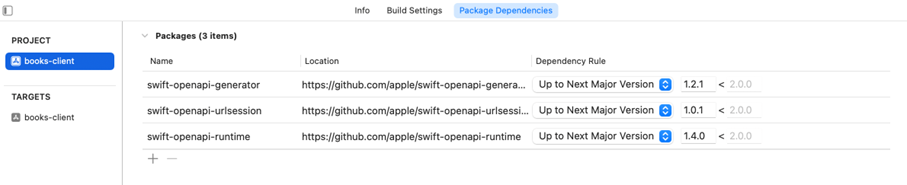
\includegraphics[scale=1.0]{../images/dependencies.png}
    \caption{Dependencies}
    
\end{figure}
\begin{figure}[htbp]
    \centering
    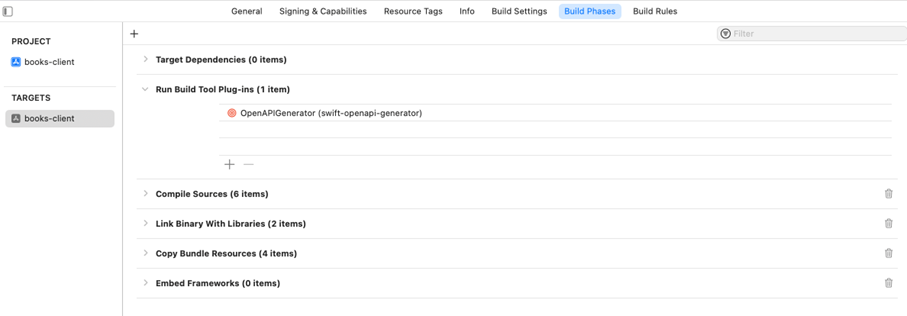
\includegraphics[scale=1.0]{../images/target.png}
    \caption{Run Build Tool Plug-ins}
    
\end{figure}



\subsubsection{Netwerklaag}
Nu wordt de netwerklaag toegevoegd aan het project. In deze netwerklaag wordt voor elk \textit{endpoint} een specifieke functie gecreëerd. Deze functies fungeren als de brug tussen de applicatie en de externe servers, waardoor communicatie mogelijk wordt via de API-\textit{endpoints}. Het bijzondere aan deze functies is dat er niet veel logica aan toegevoegd hoeft te worden. Veel van het proces wordt automatisch afgehandeld door de \textit{Client}. 
Hoewel de meeste van de logica automatisch wordt afgehandeld, moet er nog steeds aandacht moet worden besteed aan bepaalde aspecten, zoals \textit{error handling}. 
 \\ \\
De code van alle functies in de netwerklaag zijn gelijkaardig opgebouwd, daarom worden er maar twee van de vier \textit{endpoint} in detail uitgelegd. De \textit{getAllBooks} functie retourneert de automatisch gegenereerde array van de \textit{Book}-objecten van de \textit{client} of een lege array als er iets misgaat. De switch-instructie in deze functie zorgt ervoor dat we het soort gegevens terug krijgen dat we verwachten van het \textit{endpoint}. 
\begin{lstlisting}[caption=ApiService file - getAllBooks]
func getAllBooks() async -> [Components.Schemas.Book] {
    guard let response = try? await client.getAllBooks(Operations.getAllBooks.Input()) else {
        print("Error getting response")
        return []
    }
    switch response {
        case .ok(let okResponse):
            switch okResponse.body {
                case .json(let booksResponse):
                return booksResponse
            }
        case .undocumented(statusCode: let statusCode, _):
            print("Undocumented Error: \(statusCode)")
            return []
    }
}
\end{lstlisting}
De \textit{createBooks} functie gebruikt de \textit{createBook}-methode van een gegenereerde \textit{Client}-instantie, om een POST-verzoek naar een externe server te sturen, met een \textit{JSON-payload} die een nieuw boek bevat. Deze functie bevat ook de switch-instructie om na te gaan of de juiste soort gegevens terug gegeven worden. 
\begin{lstlisting}[caption=ApiService file - createBooks]
func createBooks(book: Components.Schemas.Book) async -> Components.Schemas.Book {
    guard let response = try? await client.createBook(.init(body: .json(book))) else {
        print("Error getting response")
        return Components.Schemas.Book(id: "", title: "", author: "")
    }
    switch response {
        case .created(let okResponse):
            switch okResponse.body {
                case .json(let booksResponse):
                return booksResponse
            }
        case .undocumented(statusCode: let statusCode, _):
            print("Undocumented Error: \(statusCode)")
            return Components.Schemas.Book(id: "", title: "", author: "")
        case .badRequest(_):
            print("Bad Request")
            return Components.Schemas.Book(id: "", title: "", author: "")
    }
}

\end{lstlisting}

\subsubsection{Het creëren van de views}
Wanneer de netwerklaag gemaakt is, wordt het zeer makkelijk om deze functies te gaan verwerken in je \textit{views}. Zoals hieronder in de code merkbaar is, ziet de \textit{varable @State} er vreemd uit in vergelijking met wat je anders zou gebruiken. Dit komt doordat het automatisch gegeneerde \textit{Book}-object wordt gebruikt, die is gedefinieerd in de componenten van het \textit{openapi.yaml}-bestand. In de \textit{Task modifier} wordt de netwerklaag aangeroepen om de boeken op te halen. 

\begin{lstlisting}[caption=ApiService file]
struct ContentView: View {
    @State var BooksData = [Components.Schemas.Book]()
    @Environment(\.dismiss) var dismiss
    @State private var showAddBook = false
    var body: some View {
        VStack {
            NavigationView {
                List {
                    ForEach(BooksData, id: \.id) { book in
                        NavigationLink(destination: BookView(id: book.id)) {
                            Text("\(book.title) - \(book.author)")
                        }
                    }
                }.navigationTitle("Books")
                .toolbar {
                    Button {
                        showAddBook = true
                    }label: {
                        Label("add hotspot", systemImage: "plus.circle")
                    }
                }
            }
        }
        .onAppear{
            Task {
                BooksData = await ApiService().getAllBooks()
            }
        }.sheet(isPresented: $showAddBook, onDismiss: {
            Task {
                BooksData = await ApiService().getAllBooks()
            }
        }) {
            CreateBooks()
        }
    }
}

    
\end{lstlisting}
 \newpage
 
\section{Scenario 5: aanpasbaarheid van de back-end}
Dit scenario wordt geïmplementeerd omdat het eventueel kan zijn dat er nog aanpassingen moeten gebeuren aan de back-end, nadat een \textit{client} is ontwikkeld. 
Specifiek in dit geval zou dat kunnen zijn om bijvoorbeeld extra gegevens toe te voegen aan een boek, namelijk beschrijving, \textit{genre}, … . 


\subsection{Technische doelstellingen}
Hoewel dit scenario niet bijzonder ingewikkeld is, is het cruciaal voor het onderzoeken van de flexibiliteit van een back-end die gebouwd is met de \textit{Swift OpenAPI Generator}. Deze moet in staat zijn om veranderingen in het OpenAPI-document te accommoderen. Bijvoorbeeld, als er een nieuwe \textit{client} aan het systeem wordt toegevoegd, kunnen er wijzigingen in het OpenAPI-document nodig zijn om nieuwe eisen en functionaliteiten te weerspiegelen. Dit kan variëren van het toevoegen van nieuwe \textit{endpoints} tot het wijzigen van bestaande API-specificaties.
\\ \\
Het is belangrijk om te evalueren hoe flexibel en aanpasbaar de back-end is bij het omgaan met dergelijke veranderingen. Dit omvat de mogelijkheid om snel en efficiënt updates door te voeren in de back-end code en het waarborgen van consistentie en compatibiliteit tussen de OpenAPI-specificaties en de daadwerkelijke implementatie van de API-functionaliteit.

\subsubsection{Aanpasbaarheid back-end}
Het aanpassen van de back-end gaat zeer vlot, er kunnen gemakkelijk wijzigingen gedaan worden aan het OpenAPI-document en deze kunnen gemakkelijk verwerkt worden in de \textit{handler}. Belangrijk om op te merken is dat men het model en de \textit{migration} niet mag vergeten aan te passen. Zo zijn er twee extra \textit{properties}  toegevoegd, namelijk \textit{genre} en beschrijving. 

\begin{lstlisting}[caption=openapi.yaml file]
components:
  schemas:
    Book:
      type: object
      properties:
        id:
          type: string
          format: uuid
          description: The ID of the book
        title:
          type: string
          description: The title of the book
        author:
          type: string
          description: The author of the book
        genre:
          type: string
          items:
            $ref: '#/components/schemas/Genre'
        description:
          type: string
      required:
        - id
        - title
        - author
        - genre
        - description
Genre:
  type: object
  properties:
    name:
      type: string
\end{lstlisting}

In de \textit{handler} moeten enkel de nieuwe \textit{properties} worden toegevoegd aan de functies. zoals in het onderstaand voorbeeld van de functie \textit{getAllBooks} kunt zien. 

\begin{lstlisting}[caption=handler file]
struct Handler: APIProtocol {
    ……    
    func getAllBooks(_ input: Operations.getAllBooks.Input) async throws -> Operations.getAllBooks.Output {
        let books = try await Book.query(on: app.db).all()
        logger.info("successfull GET-request to database")
        
        var booksArray: Array<Components.Schemas.Book> = []
        books.forEach { book in
            booksArray.append(Components.Schemas.Book(id: "\(String(describing: book.id))", title: book.title, author: book.author, genre: book.genre.rawValue, description: book.description))
        }
        logger.info("Converted books of database to return object")
        return .ok(.init(body: .json(booksArray)))
    }
    
}

\end{lstlisting}

\subsubsection{Aanpasbaarheid front-end}
Het aanpassen van de front-end gaat ook zeer vlot. Belangrijk om op te merken is dat het OpenAPI-document in de client overeenkomt met dat in de back-end. Hierna moet de netwerklaag nog aangepast worden naar de \textit{endpoints} of nieuwe gegevens van de \textit{components}, dit is enkel de \textit{error handling}. Dan kan gestart worden met het verwerken van de nieuwe gegevens in de UI.

\begin{lstlisting}[caption=ApiService file]
class ApiService<C: APIProtocol> {
    ...
   
    func createBooks(book: Components.Schemas.Book) async -> Components.Schemas.Book {
        guard let response = try? await client.createBook(.init(body: .json(book))) else {
            print("Error getting response")
            return Components.Schemas.Book(id: "", title: "", author: "", genre: "", description: "")
        }
        
        switch response {
            case .created(let okResponse):
            switch okResponse.body {
                case .json(let booksResponse):
                return booksResponse
            }
            case .undocumented(statusCode: let statusCode, _):
            print("Undocumented Error: \(statusCode)")
            return Components.Schemas.Book(id: "", title: "", author: "", genre: "", description: "")
            case .badRequest(_):
            print("Bad Request")
            return Components.Schemas.Book(id: "", title: "", author: "", genre: "", description: "")
        }
    }
    ...
    
}

\end{lstlisting}